\section{Aufbau}
\label{sec:Aufbau}

\begin{figure}
    \centering
    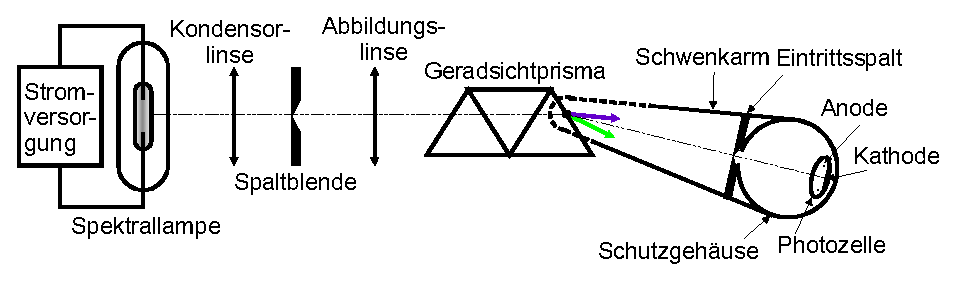
\includegraphics[height = 4cm]{Aufbau.pdf}
    \caption{Versuchsaufbau zur Untersuchung des Photoeffekts \cite{ap500}.}
    \label{fig:Aufbau}
\end{figure}
In \autoref{fig:Aufbau} ist der verwendete Versuchsaufbau gezeigt.
Es werden eine Spektrallampe, ein Aufbau zur Fokussierung des Lichtes, welcher in dem konkreten Fall aus zwei Linsen und einer Spaltblende besteht, einen Geradsichtprisma, um das Licht der Lampe in monochromatisches Licht zu teilen, und
ein Photoelement, befindlich auf einem Schwenkarm. Der Schwenkarm dient dazu, die Photozelle so auszurichten, dass jeweils nur Licht einer bestimmten Wellenlänge die Messapparatur erreicht.
Die Photozelle wird an ein Amperemeter geschlossen, sodass der Photostrom gemessen werden kann. 
Je nach angelegter Spannung wird in der Photozelle ein elektrisches Feld erzeugt, welches zur Beschleunigung oder Abbremsung freigesetzter Elektronen dient. Der genaue Aufbau ist in \autoref{fig:gegenfeld} bereits dargestellt. 